\chapter{1D Potential Wells, Stability, and Small Oscillations}
\label{ch:potential_wells}
\begin{chapterintro}
\textbf{You will learn to:} read and interpret 1D potential energy curves $E_p(x)$; determine allowed motion zones and turning points; classify equilibrium states as stable, unstable, or neutral; expand potentials in Taylor series; compute the effective stiffness $k_{\text{eff}}$; and derive the frequency of small harmonic oscillations around stable minima.
\end{chapterintro}

\section{Analysis of 1D Potential Energy Curves}

In one-dimensional motion, the conservative force is related to the potential energy $E_p(x)$ by:
\[
\boxed{F(x) = -\frac{\dd E_p}{\dd x}.}
\]
The force is the \textbf{negative slope} of the potential curve:
\begin{itemize}[leftmargin=1.4em,itemsep=2pt]
  \item If $\frac{\dd E_p}{\dd x} > 0$ (uphill slope), then $F(x) < 0$ (force pushes to the left).
  \item If $\frac{\dd E_p}{\dd x} < 0$ (downhill slope), then $F(x) > 0$ (force pushes to the right).
  \item If $\frac{\dd E_p}{\dd x} = 0$ (flat slope), then $F(x) = 0$ (\textbf{equilibrium position}).
\end{itemize}

\begin{figure}[htbp]
\centering
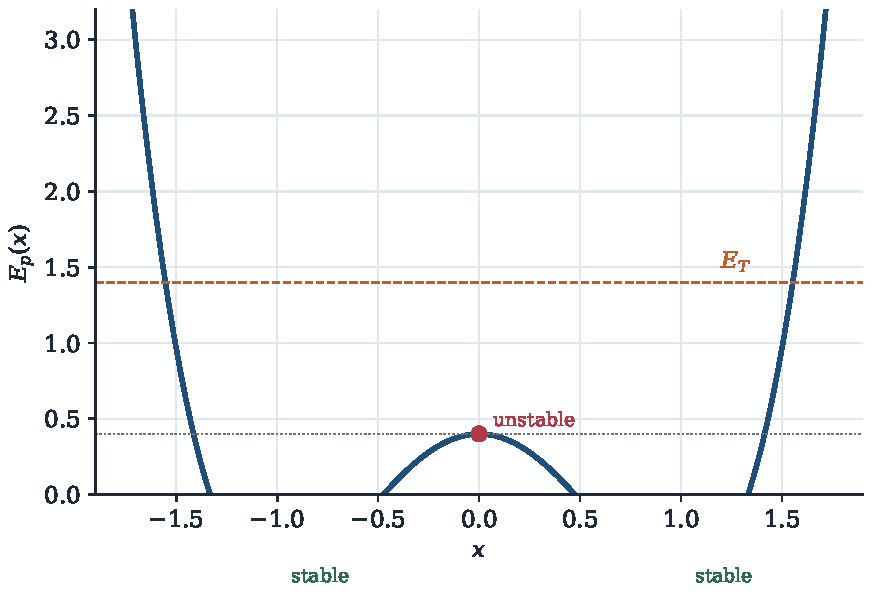
\includegraphics[width=0.74\textwidth]{figures/15_energy_well.pdf}
\caption{A one-dimensional potential energy curve $E_p(x)$ with total mechanical energy $E_m$. The particle oscillates between the classical turning points $x_1$ and $x_2$ where $E_m = E_p(x)$.}
\label{fig:energy_well}
\end{figure}

\section{Permitted Regions and Turning Points}

Since kinetic energy cannot be negative:
\[
E_c = \frac{1}{2}m v^2 = E_m - E_p(x) \ge 0 \implies \boxed{E_m \ge E_p(x).}
\]
\begin{itemize}[leftmargin=1.4em,itemsep=2pt]
  \item \textbf{Permitted region}: The set of positions where $E_p(x) \le E_m$.
  \item \textbf{Forbidden region}: Positions where $E_p(x) > E_m$ cannot be reached classically.
  \item \textbf{Turning points}: Positions $x_t$ where $E_p(x_t) = E_m$. At these points, $E_c = 0 \implies v = 0$. The particle stops and reverses direction.
  \item \textbf{Bound motion}: If the permitted region is bounded by two turning points $[x_1, x_2]$, the particle is trapped in a \textbf{potential well} and undergoes periodic oscillations.
\end{itemize}

\section{Equilibrium and Stability Criteria}

An equilibrium position $x_0$ satisfies $\left.\frac{\dd E_p}{\dd x}\right|_{x_0} = 0$. Its stability is determined by the second derivative:

\begin{center}
\renewcommand{\arraystretch}{1.3}
\begin{tabular}{@{}llll@{}}
\toprule
\textbf{Second Derivative} & \textbf{Geometry of $E_p(x)$} & \textbf{Stability} & \textbf{Restoring Force} \\
\midrule
$\left.\frac{\dd^2 E_p}{\dd x^2}\right|_{x_0} > 0$ & Local minimum (well) & \textbf{Stable} & $F \approx -k_{\text{eff}}(x-x_0)$ directed toward $x_0$ \\
$\left.\frac{\dd^2 E_p}{\dd x^2}\right|_{x_0} < 0$ & Local maximum (crest) & \textbf{Unstable} & $F \approx +k(x-x_0)$ pushes away from $x_0$ \\
$\left.\frac{\dd^2 E_p}{\dd x^2}\right|_{x_0} = 0$ & Flat inflection / plateau & \textbf{Neutral / Higher order} & Examine third and fourth derivatives \\
\bottomrule
\end{tabular}
\end{center}

\begin{figure}[htbp]
\centering
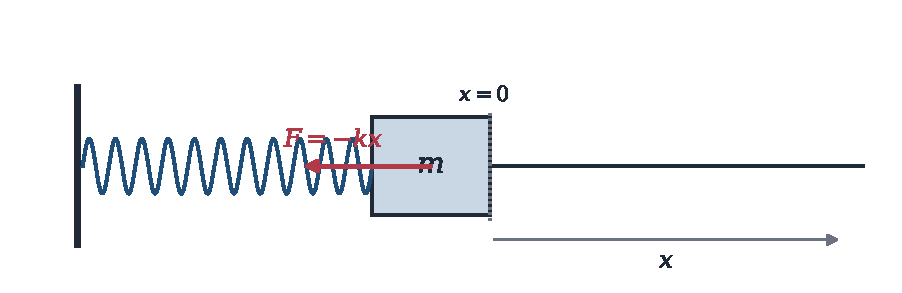
\includegraphics[width=0.68\textwidth]{figures/14_spring_mass.pdf}
\caption{The classic harmonic oscillator: a mass on a spring around its stable equilibrium position.}
\label{fig:spring_mass}
\end{figure}

\section{Small Oscillations around a Stable Minimum}

Let $x_0$ be a stable equilibrium point. Expand $E_p(x)$ in a Taylor series about $x_0$ for small displacements $\xi = x - x_0$:
\[
E_p(x) = E_p(x_0) + \underbrace{\left.\frac{\dd E_p}{\dd x}\right|_{x_0}}_{=0}\xi + \frac{1}{2}\underbrace{\left.\frac{\dd^2 E_p}{\dd x^2}\right|_{x_0}}_{\equiv k_{\text{eff}}}\xi^2 + \mathcal{O}(\xi^3).
\]
Dropping higher-order terms, the potential near the minimum is \textbf{parabolic}:
\[
\boxed{E_p(x) \approx E_p(x_0) + \frac{1}{2}k_{\text{eff}}\,\xi^2,} \quad \text{where } \boxed{k_{\text{eff}} = \left.\frac{\dd^2 E_p}{\dd x^2}\right|_{x_0} > 0.}
\]
The restoring force is linear in $\xi$:
\[
F(\xi) = -\frac{\dd E_p}{\dd\xi} \approx -k_{\text{eff}}\,\xi.
\]
Newton's second law $m\ddot{\xi} = -k_{\text{eff}}\xi$ becomes the equation of a \textbf{simple harmonic oscillator}:
\[
\boxed{\ddot{\xi} + \omega_0^2\,\xi = 0,} \quad \text{where } \boxed{\omega_0 = \sqrt{\frac{k_{\text{eff}}}{m}} = \sqrt{\left.\frac{1}{m}\frac{\dd^2 E_p}{\dd x^2}\right|_{x_0}}.}
\]
The period of small oscillations is:
\[
\boxed{T_0 = \frac{2\pi}{\omega_0} = 2\pi\sqrt{\frac{m}{k_{\text{eff}}}}.}
\]

\section{Worked Examples}

\begin{worked}[The Lennard-Jones (6-12) molecular potential]
The interaction between two noble gas atoms is modeled by the Lennard-Jones potential:
\[
U(r) = 4\epsilon\left[ \left(\frac{\sigma}{r}\right)^{12} - \left(\frac{\sigma}{r}\right)^6 \right],
\]
where $\epsilon$ is the depth of the potential well and $\sigma$ is the finite distance at which $U(\sigma) = 0$.
(a) Find the equilibrium bond length $r_0$ and the minimum potential energy $U(r_0)$.
(b) Calculate the effective spring constant $k_{\text{eff}}$ for small vibrations about $r_0$.
(c) Find the angular frequency $\omega_0$ of small vibrations for a reduced mass $\mu$.
\end{worked}

\begin{solution}{14.1}
(a) Set $\frac{\dd U}{\dd r} = 0$:
\[
\frac{\dd U}{\dd r} = 4\epsilon\left[ -12\frac{\sigma^{12}}{r^{13}} + 6\frac{\sigma^6}{r^7} \right] = \frac{24\epsilon}{r}\left[ \left(\frac{\sigma}{r}\right)^6 - 2\left(\frac{\sigma}{r}\right)^{12} \right].
\]
Setting this to zero:
\[
\left(\frac{\sigma}{r_0}\right)^6 = 2\left(\frac{\sigma}{r_0}\right)^{12} \implies \left(\frac{r_0}{\sigma}\right)^6 = 2 \implies \boxed{r_0 = 2^{1/6}\sigma \approx 1.1225\,\sigma.}
\]
The minimum potential energy is:
\[
U(r_0) = 4\epsilon\left[ \left(\frac{1}{2}\right)^2 - \frac{1}{2} \right] = 4\epsilon\left[ \frac{1}{4} - \frac{1}{2} \right] = \boxed{-\epsilon.}
\]
The dissociation energy required to separate the molecules to infinity is $\epsilon$.

(b) Compute the second derivative:
\[
\frac{\dd^2 U}{\dd r^2} = 4\epsilon\left[ 12\times 13\frac{\sigma^{12}}{r^{14}} - 6\times 7\frac{\sigma^6}{r^8} \right] = \frac{4\epsilon}{r^2}\left[ 156\left(\frac{\sigma}{r}\right)^{12} - 42\left(\frac{\sigma}{r}\right)^6 \right].
\]
Evaluating at $r = r_0$ where $(\sigma/r_0)^6 = 1/2$ and $(\sigma/r_0)^{12} = 1/4$:
\[
k_{\text{eff}} = \left.\frac{\dd^2 U}{\dd r^2}\right|_{r_0} = \frac{4\epsilon}{r_0^2}\left[ 156\left(\frac{1}{4}\right) - 42\left(\frac{1}{2}\right) \right] = \frac{4\epsilon}{r_0^2}\left[ 39 - 21 \right] = \frac{4\epsilon}{r_0^2}(18) = \boxed{\frac{72\epsilon}{r_0^2}.}
\]
Since $r_0^2 = 2^{1/3}\sigma^2$, this is $k_{\text{eff}} \approx \frac{57.14\epsilon}{\sigma^2} > 0$ (stable equilibrium!).

(c) The angular frequency of small vibrations is:
\[
\boxed{\omega_0 = \sqrt{\frac{k_{\text{eff}}}{\mu}} = \frac{1}{r_0}\sqrt{\frac{72\epsilon}{\mu}} = \frac{6}{r_0}\sqrt{\frac{2\epsilon}{\mu}}.}
\]
\end{solution}

\begin{worked}[Equilibrium and stability of a bead on an inverted parabola]
A bead of mass $m$ slides without friction on a rigid wire bent into the shape of a parabola $y = -\frac{1}{2}c x^2$ ($c > 0$) in a vertical plane, under gravity $\vec{g} = -g\jhat$.
Show that $x = 0$ is an unstable equilibrium, and find the characteristic time $\tau$ for the bead to fall away.
\end{worked}

\begin{solution}{14.2}
The potential energy of the bead in gravity is:
\[
E_p(x) = mgy = -mg\left(\frac{1}{2}c x^2\right) = -\frac{1}{2}mgc\,x^2.
\]
The first and second derivatives are:
\[
\frac{\dd E_p}{\dd x} = -mgc\,x,\qquad \frac{\dd^2 E_p}{\dd x^2} = -mgc.
\]
At $x = 0$, $\frac{\dd E_p}{\dd x} = 0$, so $x_0 = 0$ is an equilibrium point.
However:
\[
\left.\frac{\dd^2 E_p}{\dd x^2}\right|_{0} = -mgc < 0.
\]
Because the second derivative is strictly negative, the origin is a local maximum: it is an \textbf{unstable equilibrium}.
The equation of motion for small displacements ($\dot{x}^2 \ll 1 \implies \dd s \approx \dd x$) is:
\[
m\ddot{x} = -\frac{\dd E_p}{\dd x} = +mgc\,x \implies \ddot{x} - (gc)x = 0.
\]
The general solution is $x(t) = A e^{t/\tau} + B e^{-t/\tau}$ with characteristic time constant:
\[
\boxed{\tau = \frac{1}{\sqrt{gc}}.}
\]
Any tiny perturbation causes the displacement to grow exponentially with time constant $\tau$.
\end{solution}

\section{Exercises and Step-by-Step Solutions}

\begin{exercise}{\warm\ Classifying equilibria of a polynomial potential}
Consider a particle of mass $m=0.25\ \mathrm{kg}$ moving in the potential:
\[
E_p(x) = x^3 - 3x\quad (\text{with } x \text{ in metres, } E_p \text{ in joules}).
\]
(a) Find the positions of all equilibrium points.
(b) Determine the stability of each equilibrium point using the second derivative test.
(c) For the stable equilibrium point, calculate the effective spring constant $k_{\text{eff}}$ and the frequency $f_0$ of small oscillations.
\end{exercise}

\begin{tabletworkspace}[5.0cm]
\end{tabletworkspace}

\begin{solution}{14.1}
(a) Equilibria occur where $\frac{\dd E_p}{\dd x} = 0$:
\[
\frac{\dd E_p}{\dd x} = 3x^2 - 3 = 0 \implies x^2 = 1 \implies \mathbf{x_1 = -1.0\ \mathrm{m},\quad x_2 = +1.0\ \mathrm{m}.}
\]

(b) Second derivative:
\[
\frac{\dd^2 E_p}{\dd x^2} = 6x.
\]
\begin{itemize}[leftmargin=1.4em,itemsep=2pt]
  \item At $x_1 = -1.0\ \mathrm{m}$: $\left.\frac{\dd^2 E_p}{\dd x^2}\right|_{-1} = -6.0\ \mathrm{J\,m^{-2}} < 0 \implies$ \textbf{Unstable equilibrium} (local peak).
  \item At $x_2 = +1.0\ \mathrm{m}$: $\left.\frac{\dd^2 E_p}{\dd x^2}\right|_{+1} = +6.0\ \mathrm{J\,m^{-2}} > 0 \implies$ \textbf{Stable equilibrium} (local well).
\end{itemize}

(c) At the stable minimum $x_2 = 1.0\ \mathrm{m}$:
\[
k_{\text{eff}} = \left.\frac{\dd^2 E_p}{\dd x^2}\right|_{+1} = \mathbf{6.0\ \mathrm{N\,m^{-1}}.}
\]
The angular frequency is:
\[
\omega_0 = \sqrt{\frac{k_{\text{eff}}}{m}} = \sqrt{\frac{6.0}{0.25}} = \sqrt{24} \approx 4.90\ \mathrm{rad\,s^{-1}}.
\]
The oscillation frequency is:
\[
f_0 = \frac{\omega_0}{2\pi} = \frac{4.90}{2\pi} \approx \mathbf{0.78\ \mathrm{Hz}.}
\]
\end{solution}

\begin{exercise}{\warm\ Permitted regions and turning points from energy}
A particle of mass $m=1.0\ \mathrm{kg}$ moves along the $x$-axis in the potential $E_p(x) = \frac{1}{2}x^4 - 2x^2$ (in joules).
Its total mechanical energy is $E_m = -1.0\ \mathrm{J}$.
(a) Find the positions of the two potential minima and the potential barrier at $x = 0$.
(b) Find the turning points $x_t$ where $E_p(x) = E_m$.
(c) Identify the permitted intervals of motion for $E_m = -1.0\ \mathrm{J}$. Can a particle in the left well reach the right well?
\end{exercise}

\begin{tabletworkspace}[5.5cm]
\end{tabletworkspace}

\begin{solution}{14.2}
(a) Finding extrema:
\[
\frac{\dd E_p}{\dd x} = 2x^3 - 4x = 2x(x^2 - 2) = 0 \implies x = 0,\quad x = \pm\sqrt{2}.
\]
\begin{itemize}[leftmargin=1.4em,itemsep=2pt]
  \item At $x = 0$: $E_p(0) = 0\ \mathrm{J}$ (local maximum / potential barrier).
  \item At $x = \pm\sqrt{2}$: $E_p(\pm\sqrt{2}) = \frac{1}{2}(4) - 2(2) = 2 - 4 = -2.0\ \mathrm{J}$ (two symmetric minima).
\end{itemize}

(b) Turning points satisfy $E_p(x) = E_m = -1.0\ \mathrm{J}$:
\[
\frac{1}{2}x^4 - 2x^2 = -1.0 \iff x^4 - 4x^2 + 2 = 0.
\]
Let $u = x^2$:
\[
u^2 - 4u + 2 = 0 \implies u = \frac{4 \pm \sqrt{16 - 8}}{2} = 2 \pm \sqrt{2}.
\]
Since $2 - \sqrt{2} \approx 0.5858 > 0$ and $2 + \sqrt{2} \approx 3.4142$:
\[
x = \pm\sqrt{2 - \sqrt{2}} \approx \pm 0.765\ \mathrm{m},\qquad x = \pm\sqrt{2 + \sqrt{2}} \approx \pm 1.848\ \mathrm{m}.
\]

(c) The condition $E_p(x) \le E_m = -1.0\ \mathrm{J}$ requires:
\[
\text{Left well:}\quad x \in [-1.848\ \mathrm{m},\ -0.765\ \mathrm{m}], \qquad \text{Right well:}\quad x \in [+0.765\ \mathrm{m},\ +1.848\ \mathrm{m}].
\]
The interval $(-0.765\ \mathrm{m}, +0.765\ \mathrm{m})$ is classically \textbf{forbidden} because $E_p(x) > -1.0\ \mathrm{J}$ there (with a peak of $0\ \mathrm{J}$ at $x=0$).
Therefore, a classical particle starting in the left well is trapped forever and \textbf{cannot reach the right well} (in quantum mechanics, it could tunnel through).
\end{solution}

\begin{exercise}{\core\ The Morse potential for molecular bonds}
The potential energy between two atoms in a diatomic molecule (such as $\mathrm{HCl}$) is well approximated by the Morse potential:
\[
V(r) = D_e\left[ 1 - e^{-a(r - r_e)} \right]^2,
\]
where $D_e$ is the well depth, $r_e$ is the equilibrium separation, and $a$ is the width parameter.
(a) Verify that $r = r_e$ is the equilibrium separation and find $V(r_e)$.
(b) Compute the effective spring constant $k_{\text{eff}} = \left.\frac{\dd^2 V}{\dd r^2}\right|_{r_e}$.
(c) For $\mathrm{HCl}$, $D_e = 4.43\ \mathrm{eV} = 7.10\times 10^{-19}\ \mathrm{J}$, $a = 1.90\times 10^{10}\ \mathrm{m^{-1}}$, and reduced mass $\mu = 1.63\times 10^{-27}\ \mathrm{kg}$. Calculate $k_{\text{eff}}$ and the vibrational frequency $\nu = \omega_0 / 2\pi$.
\end{exercise}

\begin{tabletworkspace}[6.0cm]
\end{tabletworkspace}

\begin{solution}{14.3}
(a) First derivative:
\[
\frac{\dd V}{\dd r} = 2D_e\left[ 1 - e^{-a(r - r_e)} \right]\left[ a e^{-a(r - r_e)} \right] = 2a D_e e^{-a(r - r_e)}\left[ 1 - e^{-a(r - r_e)} \right].
\]
At $r = r_e$:
\[
\left.\frac{\dd V}{\dd r}\right|_{r_e} = 2a D_e(1)(1 - 1) = 0.
\]
Thus $r_e$ is indeed an equilibrium position.
The potential energy at equilibrium is $V(r_e) = D_e(1 - 1)^2 = \mathbf{0\ \mathrm{J}}$.

(b) Second derivative:
\begin{align*}
\frac{\dd^2 V}{\dd r^2} &= 2a D_e \frac{\dd}{\dd r}\left[ e^{-a(r - r_e)} - e^{-2a(r - r_e)} \right] \\
&= 2a D_e\left[ -a e^{-a(r - r_e)} + 2a e^{-2a(r - r_e)} \right] = 2a^2 D_e\left[ 2e^{-2a(r - r_e)} - e^{-a(r - r_e)} \right].
\end{align*}
Evaluating at $r = r_e$:
\[
k_{\text{eff}} = \left.\frac{\dd^2 V}{\dd r^2}\right|_{r_e} = 2a^2 D_e(2 - 1) = \boxed{2a^2 D_e.}
\]

(c) Numerical values:
\[
k_{\text{eff}} = 2(1.90\times 10^{10})^2\times(7.10\times 10^{-19}) = 2(3.61\times 10^{20})\times(7.10\times 10^{-19}) = \mathbf{512.6\ \mathrm{N\,m^{-1}}.}
\]
Vibrational angular frequency:
\[
\omega_0 = \sqrt{\frac{k_{\text{eff}}}{\mu}} = \sqrt{\frac{512.6}{1.63\times 10^{-27}}} = \sqrt{3.145\times 10^{29}} \approx 5.61\times 10^{14}\ \mathrm{rad\,s^{-1}}.
\]
Vibrational frequency:
\[
\nu = \frac{\omega_0}{2\pi} = \frac{5.61\times 10^{14}}{2\pi} \approx \mathbf{8.93\times 10^{13}\ \mathrm{Hz}} = 89.3\ \mathrm{THz}.
\]
(This corresponds to an infrared absorption wavelength $\lambda = c/\nu \approx 3.36\ \mu\mathrm{m}$, typical of molecular vibration).
\end{solution}

\begin{exercise}{\core\ Oscillations of a floating cylinder}
A uniform solid vertical cylinder of mass $m$, radius $R$, and length $H$ floats upright in a liquid of density $\rho$ ($\rho > m / (\pi R^2 H)$).
Let $z$ be the downward vertical displacement from its static equilibrium floating position.
(a) Determine the equilibrium submerged depth $h_0$.
(b) Show that the net restoring force for a small displacement $z$ is $F_z = -(\rho g \pi R^2)z$.
(c) Derive the effective potential energy $E_p(z)$ and show that the vertical bobbing frequency is $\omega_0 = \sqrt{\frac{g}{h_0}}$.
\end{exercise}

\begin{tabletworkspace}[5.5cm]
\end{tabletworkspace}

\begin{solution}{14.4}
(a) At static equilibrium, Archimedes' buoyant force balances gravity:
\[
F_B = \rho g V_{\text{sub}} = \rho g (\pi R^2 h_0) = mg \implies \boxed{h_0 = \frac{m}{\rho \pi R^2}.}
\]

(b) When the cylinder is displaced downward by $z$, the submerged depth increases to $h_0 + z$.
The buoyant force becomes $F_B(z) = \rho g \pi R^2(h_0 + z)$.
The net vertical force (with downward positive) is:
\[
F_{\text{net}} = mg - F_B(z) = mg - \rho g \pi R^2 h_0 - \rho g \pi R^2 z.
\]
Using $mg = \rho g \pi R^2 h_0$, the static terms cancel:
\[
\boxed{F_{\text{net}}(z) = -(\rho g \pi R^2)\,z.}
\]
The restoring force is purely linear (Hookean)!

(c) Potential energy:
\[
E_p(z) = -\int_0^z F_{\text{net}}(z')\dd z' = \frac{1}{2}(\rho g \pi R^2)z^2.
\]
Since $\frac{\dd^2 E_p}{\dd z^2} = \rho g \pi R^2 = k_{\text{eff}} > 0$, the equilibrium is unconditionally stable.
Newton's second law gives:
\[
m\ddot{z} + (\rho g \pi R^2)z = 0 \implies \ddot{z} + \omega_0^2 z = 0,
\]
with angular frequency:
\[
\omega_0 = \sqrt{\frac{\rho g \pi R^2}{m}}.
\]
Substituting $m = \rho \pi R^2 h_0$:
\[
\boxed{\omega_0 = \sqrt{\frac{g}{h_0}}.}
\]
Remarkably, the bobbing frequency of any floating cylinder depends solely on its submerged depth $h_0$, identical to a simple pendulum of length $L = h_0$!
\end{solution}

\begin{exercise}{\mastery\ Mass between two pre-tensioned transverse springs}
A particle of mass $m$ can slide along a smooth horizontal $x$-axis. It is held between two identical horizontal springs perpendicular to the $x$-axis, each of spring constant $k$ and natural length $\ell_0$, attached to fixed posts at $(0, +d)$ and $(0, -d)$ with $d > \ell_0$ (pre-tensioned).
(a) Express the total potential energy $E_p(x)$ of the two springs as a function of the transverse displacement $x$.
(b) Expand $E_p(x)$ in powers of $x$ up to order $x^4$.
(c) Find the effective spring constant $k_{\text{eff}}$ at $x = 0$ and the frequency $\omega_0$ of small oscillations.
(d) What happens if the posts are moved to $d = \ell_0$ (unstretched at $x=0$) or $d < \ell_0$ (compressed)?
\end{exercise}

\begin{tabletworkspace}[6.5cm]
\end{tabletworkspace}

\begin{solution}{14.5}
(a) The distance from the mass at $(x, 0)$ to either post at $(0, \pm d)$ is $\ell(x) = \sqrt{x^2 + d^2}$.
The extension of each spring is $\Delta\ell = \ell(x) - \ell_0 = \sqrt{x^2 + d^2} - \ell_0$.
The total potential energy of both identical springs is:
\[
\boxed{E_p(x) = 2\times\frac{1}{2}k\left( \sqrt{x^2 + d^2} - \ell_0 \right)^2 = k\left( \sqrt{x^2 + d^2} - \ell_0 \right)^2.}
\]

(b) For small displacements $x \ll d$:
\[
\sqrt{x^2 + d^2} = d\sqrt{1 + \frac{x^2}{d^2}} \approx d\left( 1 + \frac{1}{2}\frac{x^2}{d^2} - \frac{1}{8}\frac{x^4}{d^4} \right).
\]
The extension is:
\[
\sqrt{x^2 + d^2} - \ell_0 \approx (d - \ell_0) + \frac{x^2}{2d} - \frac{x^4}{8d^3}.
\]
Squaring this:
\begin{align*}
E_p(x) &\approx k\left[ (d - \ell_0)^2 + 2(d - \ell_0)\frac{x^2}{2d} + \frac{x^4}{4d^2} - 2(d - \ell_0)\frac{x^4}{8d^3} \right] \\
&= k(d - \ell_0)^2 + k\left(1 - \frac{\ell_0}{d}\right)x^2 + \frac{k\ell_0}{4d^3}x^4.
\end{align*}

(c) The linear restoring term corresponds to the coefficient of $\frac{1}{2}x^2$:
\[
\frac{1}{2}k_{\text{eff}} = k\left(1 - \frac{\ell_0}{d}\right) \implies \boxed{k_{\text{eff}} = 2k\left(1 - \frac{\ell_0}{d}\right).}
\]
Since $d > \ell_0$, $k_{\text{eff}} > 0$: the equilibrium at $x = 0$ is \textbf{stable}.
The angular frequency of small transverse oscillations is:
\[
\boxed{\omega_0 = \sqrt{\frac{2k}{m}\left(1 - \frac{\ell_0}{d}\right)}.}
\]

(d) Physical discussion of regimes:
\begin{itemize}[leftmargin=1.4em,itemsep=2pt]
  \item If $d = \ell_0$ (unstretched at $x=0$): $k_{\text{eff}} = 0$. The harmonic term vanishes! The potential becomes quartic: $E_p(x) \approx \frac{k}{4d^2}x^4$. The restoring force is non-linear ($F \propto -x^3$), and the oscillation frequency depends on amplitude!
  \item If $d < \ell_0$ (springs compressed at $x=0$): $k_{\text{eff}} < 0$. The origin $x = 0$ becomes \textbf{unstable}! The compressed springs buckle to the left or right, creating two new symmetric stable equilibrium points at $x_e = \pm\sqrt{\ell_0^2 - d^2}$.
\end{itemize}
\end{solution}
